\documentclass[border=8pt]{standalone}
\usepackage{lmodern}
\usepackage[T1]{fontenc}
\usepackage{amsmath,amssymb}
\usepackage{tikz}
\begin{document}
% Text flowing around a figure, by hand: \parshape narrows the first k
% lines, and the figure hangs from the first baseline in a zero-width box.
\newdimen\W \W=11.5cm      % the measure
\newdimen\F \F=4.4cm       % width reserved for the figure
\newcount\k \k=9           % lines beside it
\def\shape{}\newcount\i \i=1
\loop \edef\shape{\shape 0pt \the\dimexpr\W-\F\relax\space}\advance\i 1 \ifnum\i<\numexpr\k+1\relax\repeat
\edef\shape{\shape 0pt \the\W}
\vtop{\hsize=\W \parindent=0pt \tolerance=2000 \emergencystretch=1em
  \parshape \numexpr\k+1\relax \shape
  % \vtop{\kern0pt ...} puts the whole picture below the baseline; \smash hides
  % that depth from the line spacing; \raise lines its top up with the first line.
  \rlap{\hskip\dimexpr\W-\F+3mm\relax\smash{\raise\ht\strutbox\vtop{\kern0pt\hbox{%
    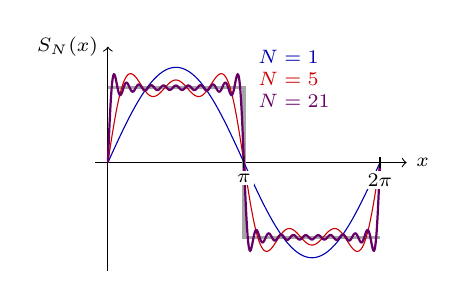
\begin{tikzpicture}[x=0.55cm,y=0.95cm,font=\scriptsize]
      \draw[->] (-0.3,0) -- (6.9,0) node[right] {$x$};
      \draw[->] (0,-1.45) -- (0,1.55) node[left] {$S_N(x)$};
      \draw[gray!70,line width=1.2pt] (0,1) -- (3.1416,1) -- (3.1416,-1) -- (6.2832,-1);
      \draw[blue!70!black,domain=0:6.2832,samples=90] plot (\x,{4/pi*sin(\x r)});
      \draw[red!80!black,domain=0:6.2832,samples=200] plot (\x,{4/pi*(sin(\x r)+sin(3*\x r)/3+sin(5*\x r)/5)});
      \draw[violet!80!black,thick,domain=0:6.2832,samples=500] plot (\x,{4/pi*(sin(\x r)+sin(3*\x r)/3+sin(5*\x r)/5+sin(7*\x r)/7+sin(9*\x r)/9+sin(11*\x r)/11+sin(13*\x r)/13+sin(15*\x r)/15+sin(17*\x r)/17+sin(19*\x r)/19+sin(21*\x r)/21)});
      \foreach \t/\l in {3.1416/$\pi$,6.2832/$2\pi$} \draw (\t,2pt) -- (\t,-2pt) node[below=1pt,fill=white,inner sep=1pt] {\l};
      \node[anchor=north west,align=left,inner sep=1pt] at (3.4,1.55) {\textcolor{blue!70!black}{$N=1$}\\ \textcolor{red!80!black}{$N=5$}\\ \textcolor{violet!80!black}{$N=21$}};
    \end{tikzpicture}}}}}%
  Any reasonable periodic function is a sum of sines and cosines. For the square wave
  \tikz[baseline=-0.5ex]\draw (0,-0.7ex)--(0,0.7ex)--(0.9em,0.7ex)--(0.9em,-0.7ex)--(1.8em,-0.7ex);
  $f(x)=\operatorname{sgn}(\sin x)$ the cosine coefficients
  $a_n=\frac1\pi\int_{-\pi}^{\pi}f(x)\cos nx\,dx$ all vanish, while
  $b_n=\frac{2}{\pi n}\,(1-\cos n\pi)$, so only the odd harmonics survive:
  \[ f(x)=\frac{4}{\pi}\sum_{k=0}^{\infty}\frac{\sin\bigl((2k+1)x\bigr)}{2k+1}. \]
  The partial sums $S_N$ on the right overshoot each jump by about nine per cent
  however large $N$ becomes: the Gibbs phenomenon,
  $\lim_{N\to\infty}S_N\!\left(\tfrac{\pi}{2N}\right)=\tfrac{2}{\pi}\operatorname{Si}(\pi)\approx1.179$.
  Parseval's identity $\frac1\pi\int_{-\pi}^{\pi}f^2=\sum_n b_n^2$ then yields
  $\sum_{k\ge0}(2k+1)^{-2}=\pi^2/8$, from which Euler's $\zeta(2)=\pi^2/6$ follows in one line.
  The gap the text flows around is a \texttt{\char`\\parshape} too: nine narrow lines beside the
  figure, then the full measure, with the figure itself hung from the first baseline in a
  zero-width \texttt{\char`\\rlap} box.\par}
\end{document}
